\documentclass[10pt]{beamer}

\usetheme[subsectionpage=progressbar]{metropolis}
\usepackage{appendixnumberbeamer}

\usepackage{ucs}
\usepackage[utf8x]{inputenc}
\usepackage[ngerman]{babel}

\usepackage{booktabs}
\usepackage[scale=2]{ccicons}

\usepackage{pgfplots}
\usepgfplotslibrary{dateplot}

\usepackage{xspace}
\usepackage{dsfont}
\usepackage{graphicx}
\newcommand{\themename}{\textbf{\textsc{metropolis}}\xspace}

\usepackage{caption}
\usepackage{subcaption}

\title{Nummernschilderkennung mit Python}
% \subtitle{Machine Learning in Produktion und Logistik}
\date{18. Februar 2021}
\author{Anne-Sophie Bollmann, Susanne Kl\"ocker, Pia von Kolken, Christian Peters}
%\institute{TU Dortmund}
%\titlegraphic{\hfill\includegraphics[height=1.5cm]{logo.pdf}}

\begin{document}

\maketitle

\section{Pipeline}

\begin{frame}{Pipeline}
  \begin{figure}
    \begin{center}
      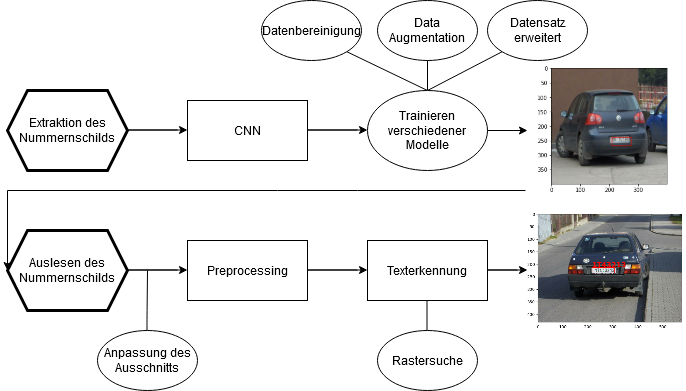
\includegraphics[width=0.8\textwidth]{img/Pipeline}
      \caption{Beschreibung\footnote{Bildquelle: \url{https://github.com/theAIGuysCode/yolov4-custom-functions}}}
    \end{center}
  \end{figure}
\end{frame}


\section{Image Segmentation}

\begin{frame}{Trainingseingaben}
    \begin{figure}
        \centering
        \begin{subfigure}{0.495\textwidth}
            \centering
            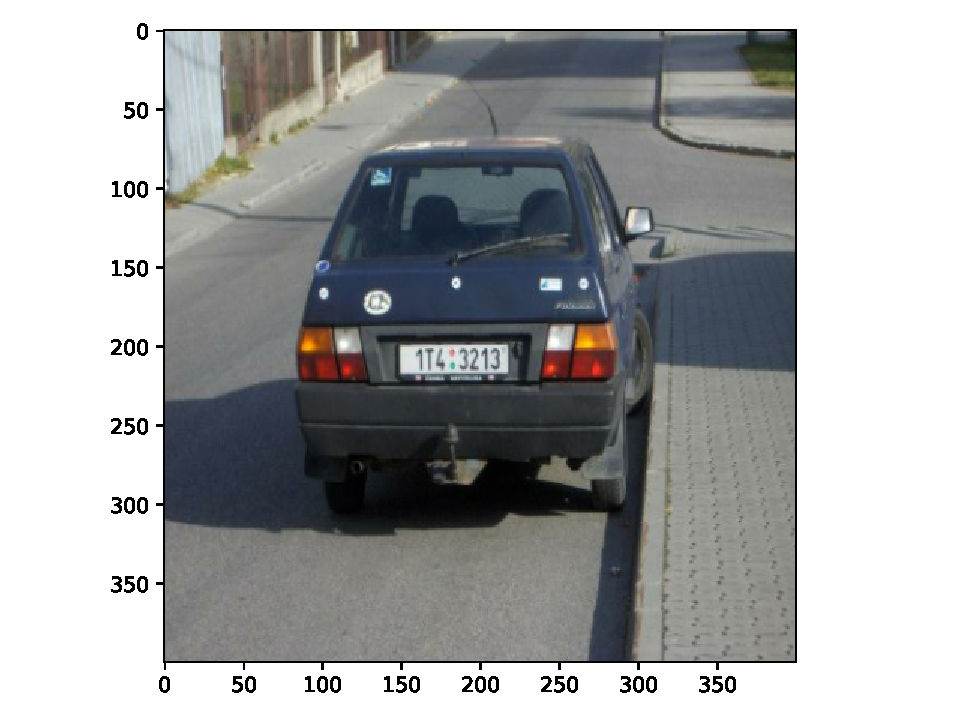
\includegraphics[width=\textwidth]{img/model_demo_1}
            \caption{Eingabe}
        \end{subfigure}
        \begin{subfigure}{0.495\textwidth}
            \centering
            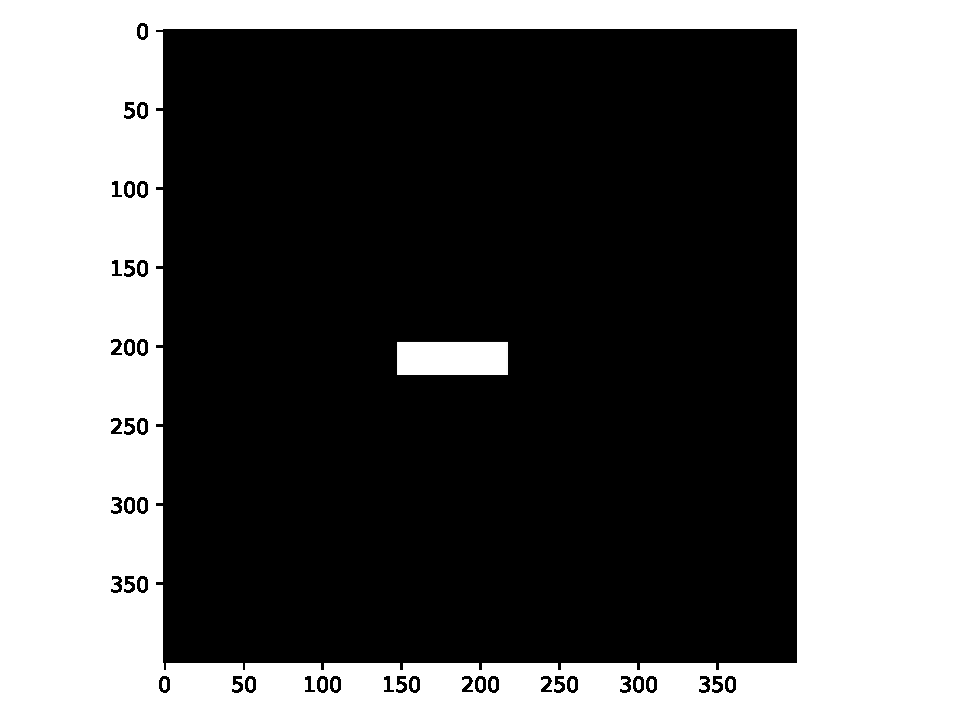
\includegraphics[width=\textwidth]{img/model_demo_2}
            \caption{Ziel}
        \end{subfigure}
    \end{figure}
\end{frame}

\begin{frame}{Modellarchitektur}
    \begin{figure}
        \centering
        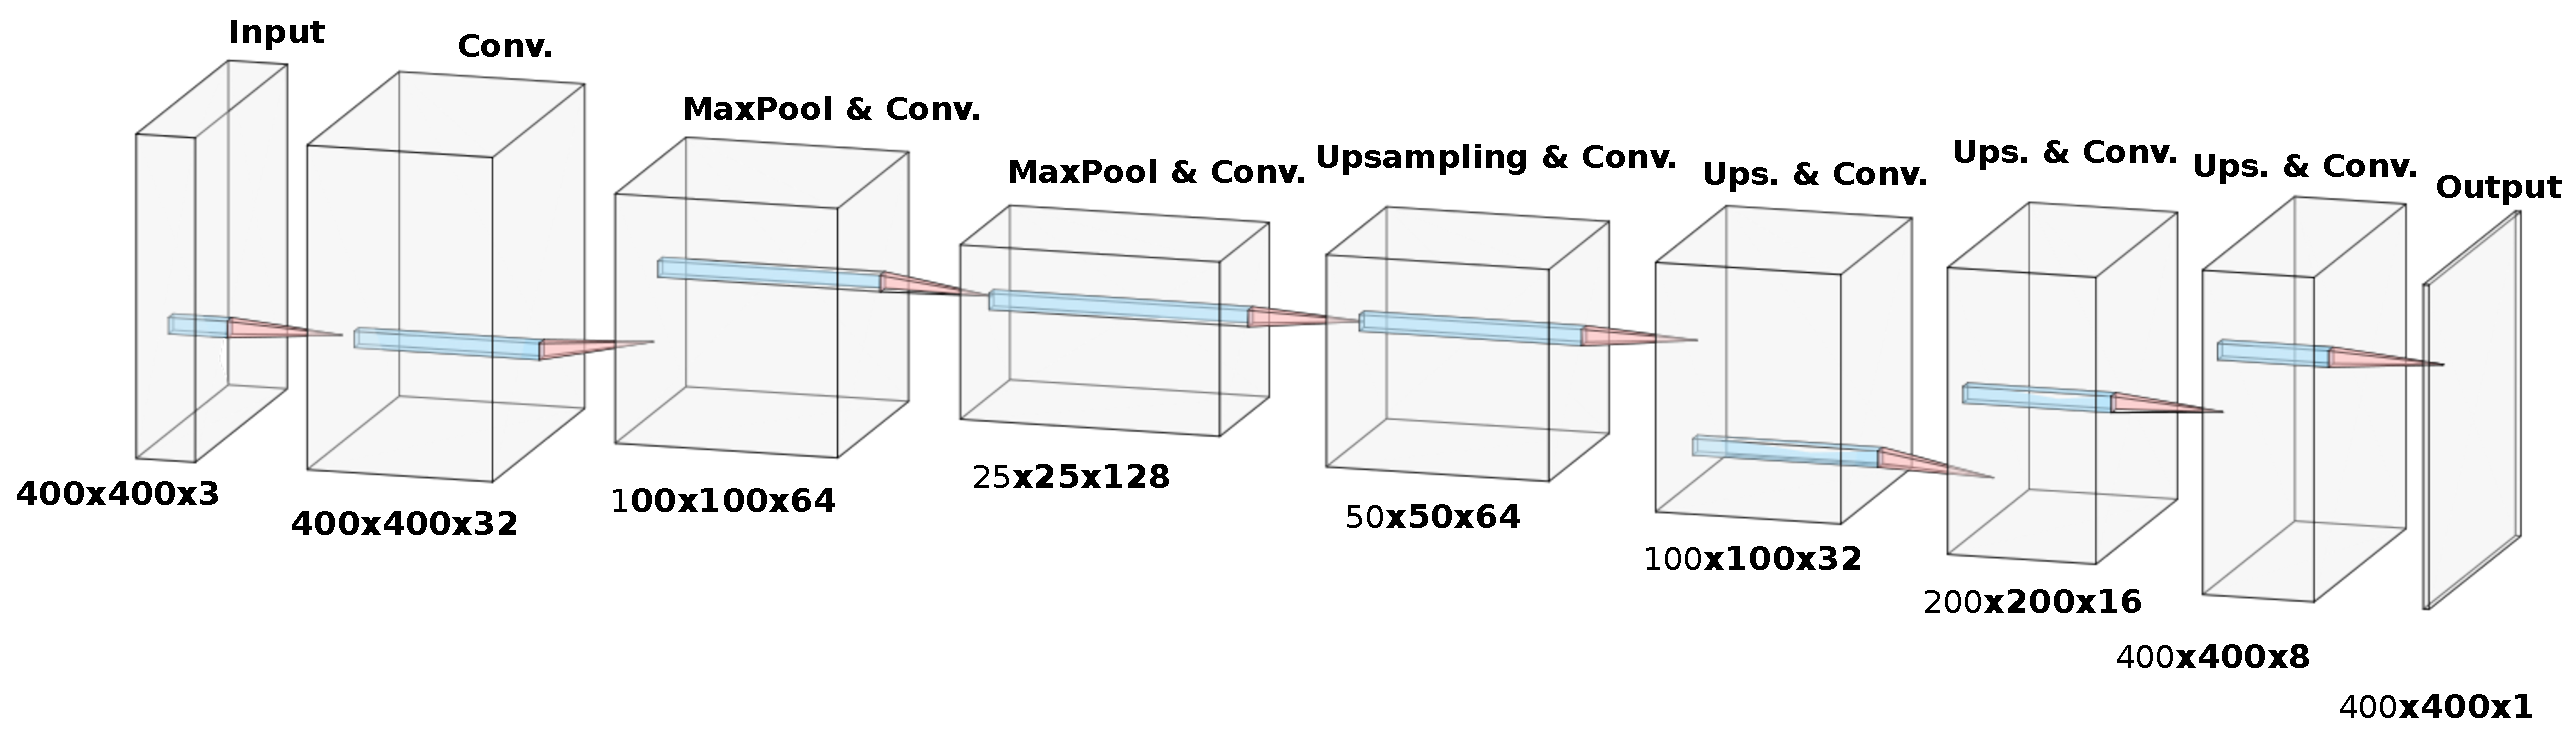
\includegraphics[width=\textwidth]{img/nn.pdf}
        \caption{Das Ergebnis nach wochenlangem Ausprobieren. Insgesamt 191.297 trainierbare Parameter.}
    \end{figure}
\end{frame}

\begin{frame}{Modellvorhersage}
    \begin{figure}
        \centering
        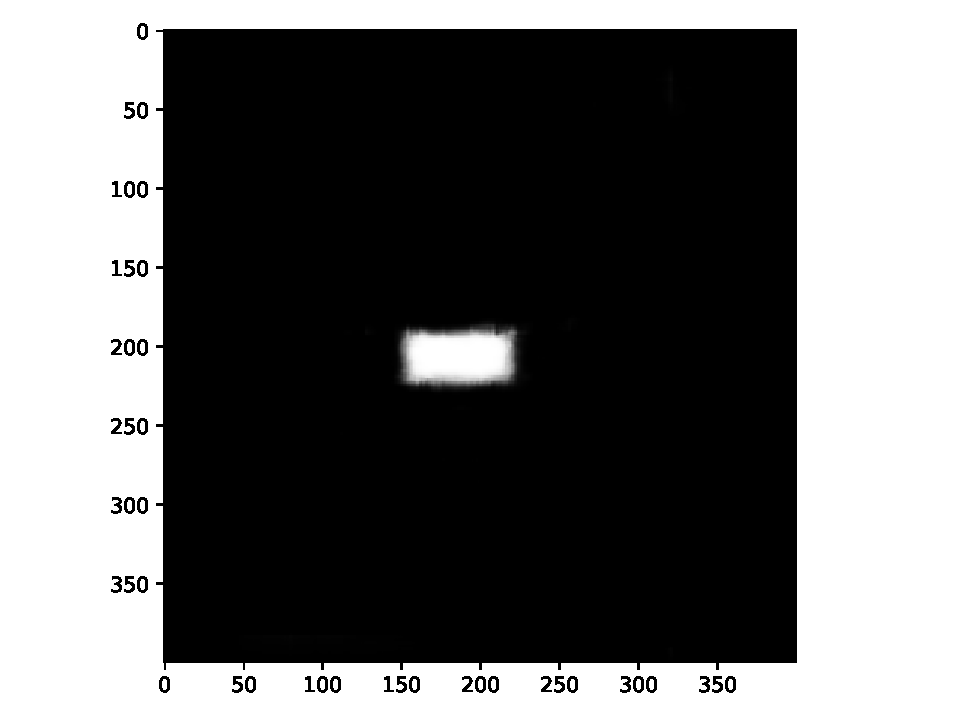
\includegraphics[width=0.9\textwidth]{img/model_demo_3}
    \end{figure}
\end{frame}

\begin{frame}{Schwellenwert}
    \begin{figure}
        \centering
        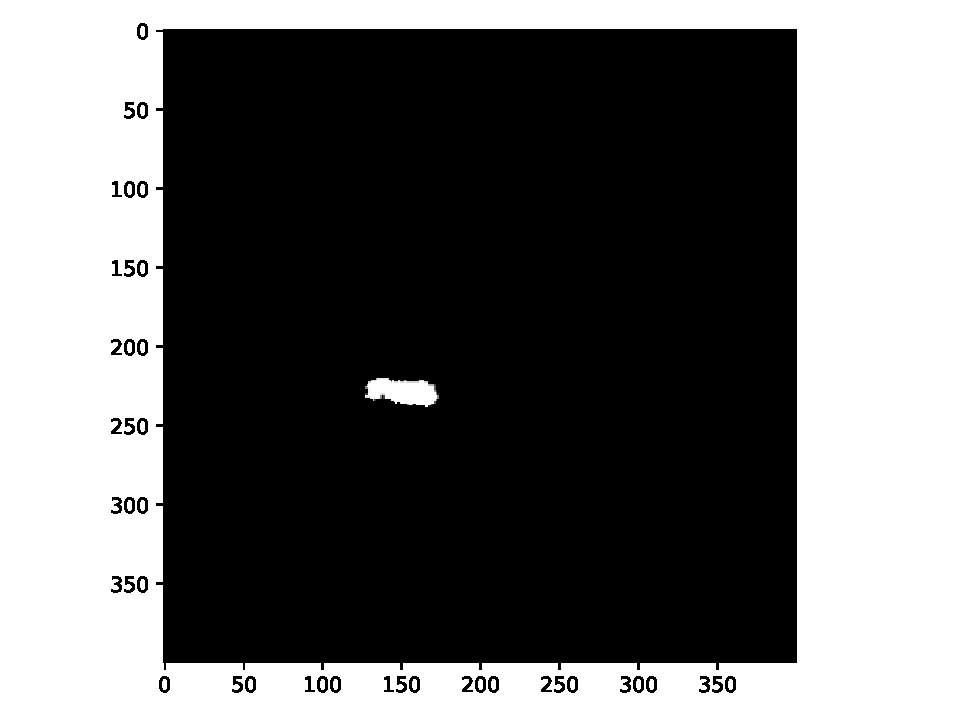
\includegraphics[width=0.9\textwidth]{img/model_demo_4}
    \end{figure}
\end{frame}

\begin{frame}{Umschlie{\ss}endes Rechteck}
    \begin{figure}
        \centering
        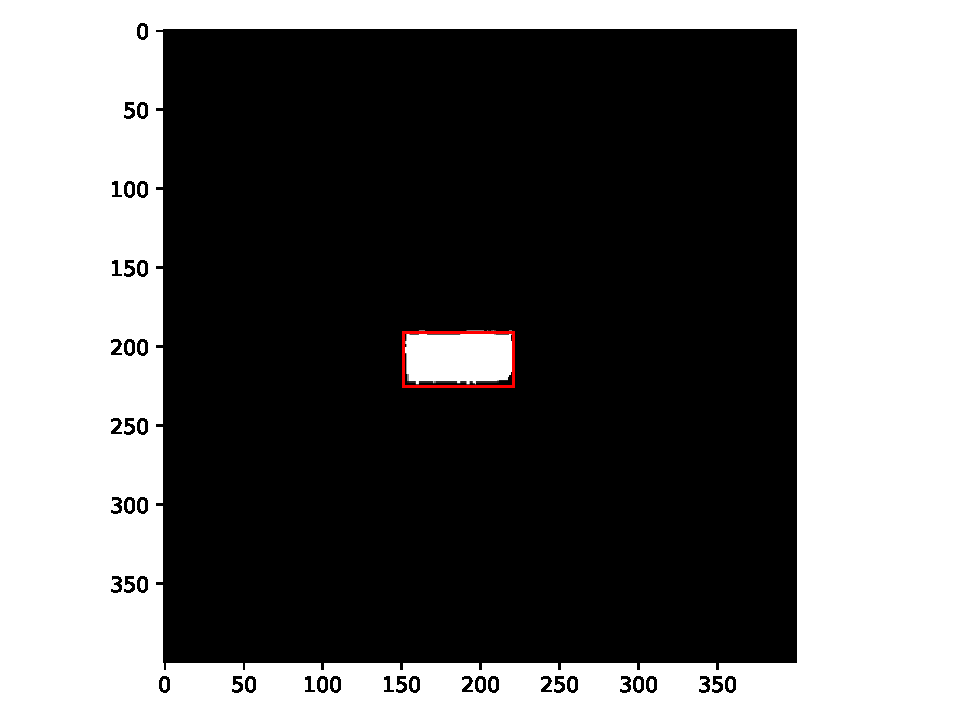
\includegraphics[width=0.9\textwidth]{img/model_demo_5}
    \end{figure}
\end{frame}

\begin{frame}{Resultat}
    \begin{figure}
        \centering
        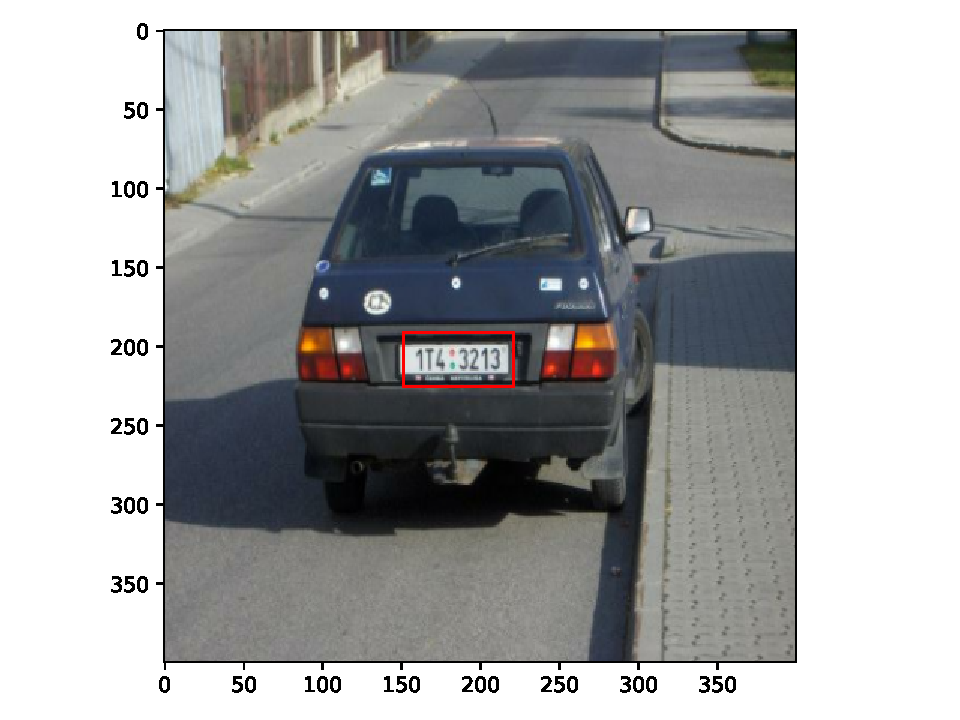
\includegraphics[width=0.9\textwidth]{img/model_demo_6}
    \end{figure}
\end{frame}

\begin{frame}{Details zum Training}
    \textbf{Implementierung in Tensorflow, Training auf Google Colab GPU}
    \begin{itemize}
        \item 534 Zus\"atzliche Trainingsbilder hinzugef\"ugt\footnote{\url{https://github.com/RobertLucian/license-plate-dataset}}
        \item Data Augmentation: $949 \Rightarrow 22.776$ Bilder
              \begin{itemize}
                  \item Horizontal Flip, Random Cropping, Random Contrast, Random Brightness
                  \item \textbf{Ben\"otigt $>$14GB GPU Speicher!}
              \end{itemize}
        \item Mini Batch Stochastic Gradient Descent mit ADAM Optimizer
        \item Loss: Binary cross entropy
              \begin{equation*}
                  -\sum_{i \in \text{Pixel}} y_{true}^{(i)} \log (y_{pred}^{(i)}) + (1 - y_{true}^{(i)}) \log (1 - y_{pred}^{(i)})
              \end{equation*}
        \item Zur Validierung 20 Bilder aus EU/RO per Hand selektiert
        \item \glqq Early Stopping\grqq{} nach 19 Epochen
    \end{itemize}
\end{frame}


\section{Optical Character Recognition}

\begin{frame}{Bearbeitungsschritte}
\begin{columns}
\begin{column}{0.6\textwidth}
\begin{enumerate}
\item {\small Vergr\"osserung und Graustufen}
\item {\small Blurring (Bildgl\"attung)}
\item[-] {\scriptsize Gaußsche Unsch\"arfe und Median Unsch\"arfe}
\item {\small Thresholding (Schwellenwertverfahren)}

\item[-] {\scriptsize Otsu: w\"ahlt automatisch einen geeigneten Schwellenwert aus}
\item[-] {\scriptsize Einfaches Verfahren mit Schwellenwerten $\{60,80,100,120\}$}
\item[-] {\scriptsize Binary-Inv.: Die Werte derart getauscht, dass schwarz zu weiß wird und umgekehrt $\rightarrow$ führt zur besseren Erkennung von Konturen}

\item {\small Dilation (Morphologische Transformation)}
\end{enumerate}
\end{column}
\begin{column}{0.40\textwidth}
    \begin{center}
        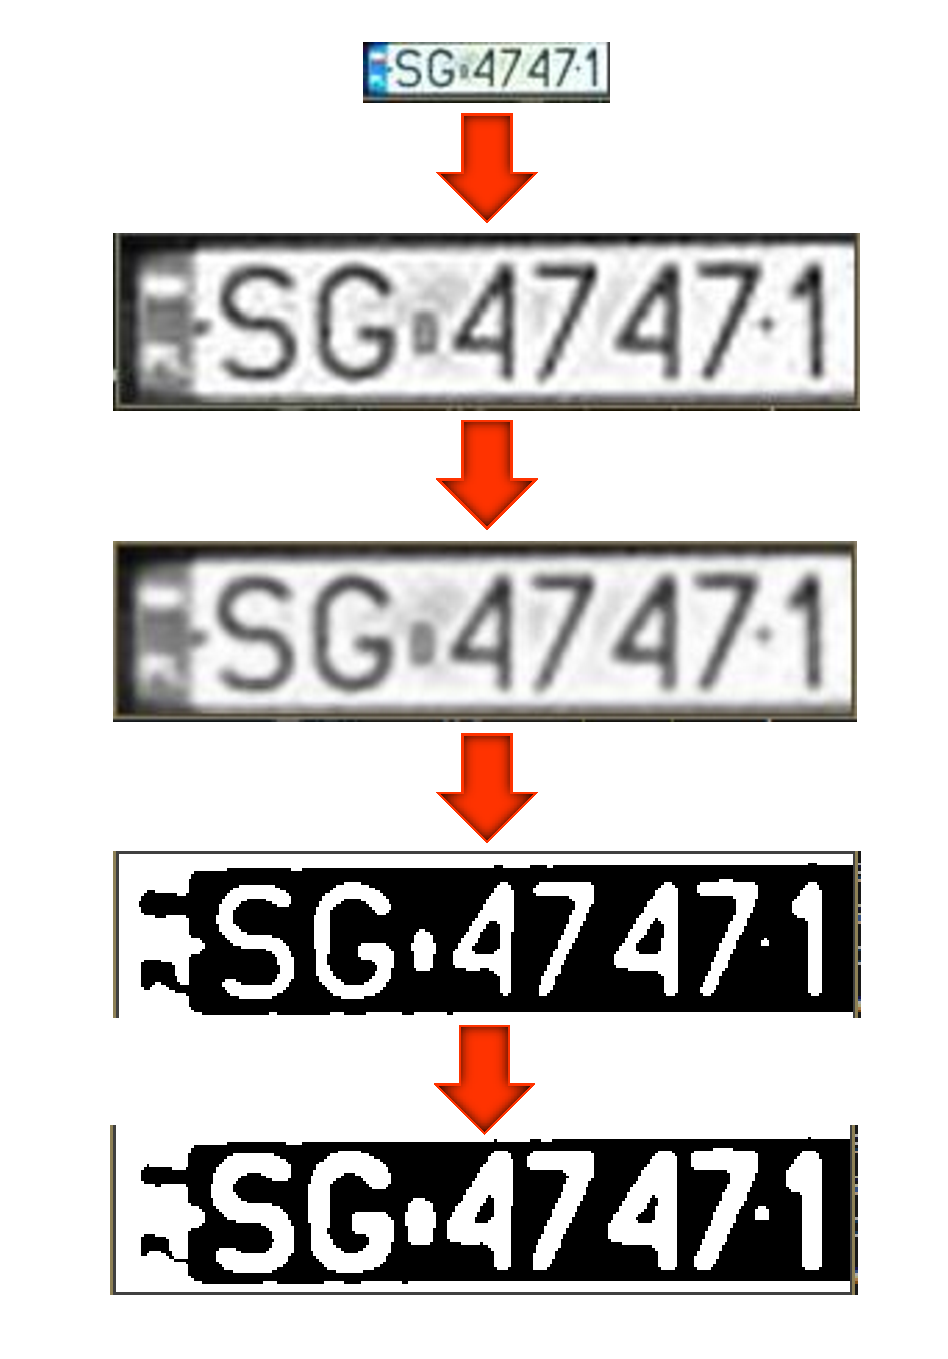
\includegraphics[width=\textwidth]{img/preprocessing}
    \end{center}
\end{column}
\end{columns}
\end{frame}

\begin{frame}{Aussortierung der Konturen}
\begin{itemize}
\item {\textit{\scriptsize Genutzt werden die Werte x, y, w, h (Werte der Kontur) sowie width und height (Breite und Höhe des Bildes)}}
\item {\scriptsize Es werden nur Konturen berücksichtigt, die folgende Bedingungen erf\"ullen:}
\end{itemize}
\begin{align*}
    \frac{height}{h} > 3
    \hspace{1cm}
    \frac{h}{w} < 1.2
    \hspace{1cm}
    \frac{width}{w} > 50
\end{align*}
    \begin{center}
        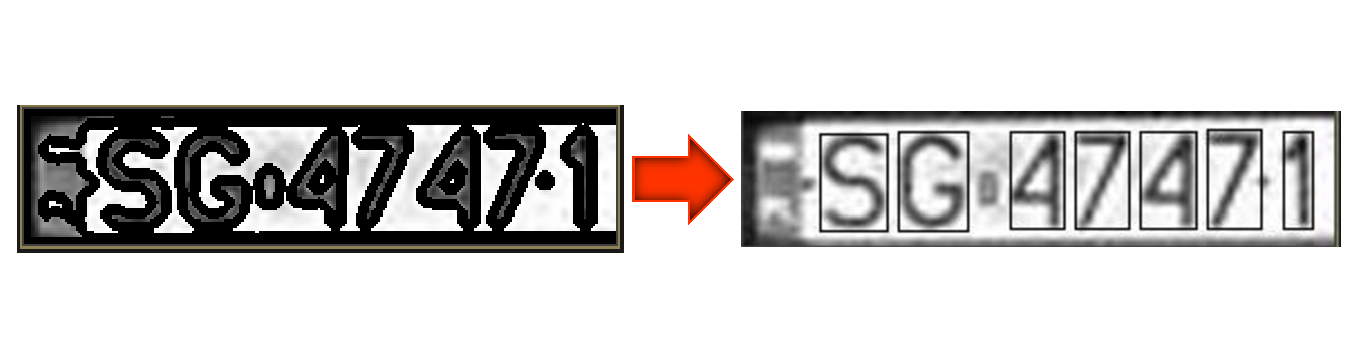
\includegraphics[width=\textwidth]{img/contours}
    \end{center}
\end{frame}

\begin{frame}{Character auslesen}

{\footnotesize Einstellungen für das Auslesen mit Tesseract 5:}
\begin{itemize}
\item {\scriptsize Jeder Character wird einzeln ausgelesen \rightarrow  \, Page Segmentation Mode (\texttt{--psm10})}
\item {\scriptsize Engine Mode \texttt{--oem3}}
\item {\scriptsize Zeichen-Whitelist (Großbuchstaben + Zahlen 0-9)}
\item {\scriptsize Außerdem: Bild darf nicht zu nahe am Character ausgeschnitten werden}

\begin{center}
    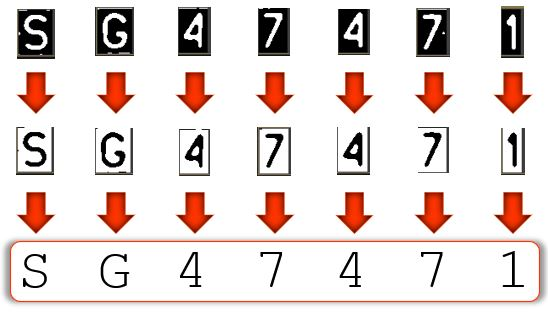
\includegraphics[width=0.75\textwidth]{img/char_preprocessing.jpg}
\end{center}

\end{itemize}
\end{frame}


\begin{frame}{Boundingboxes verschieben und Levenshtein-Distanz}
Falls keine Character in der gefundenen Bounding-Box erkannt werden, verschiebe die Bounding-Box anhand unterschiedlicher Methoden: {\textit{hoch, runter, rechts, links, oben-rechts, unten-rechts, unten-links, oben-links}}
\begin{center}
    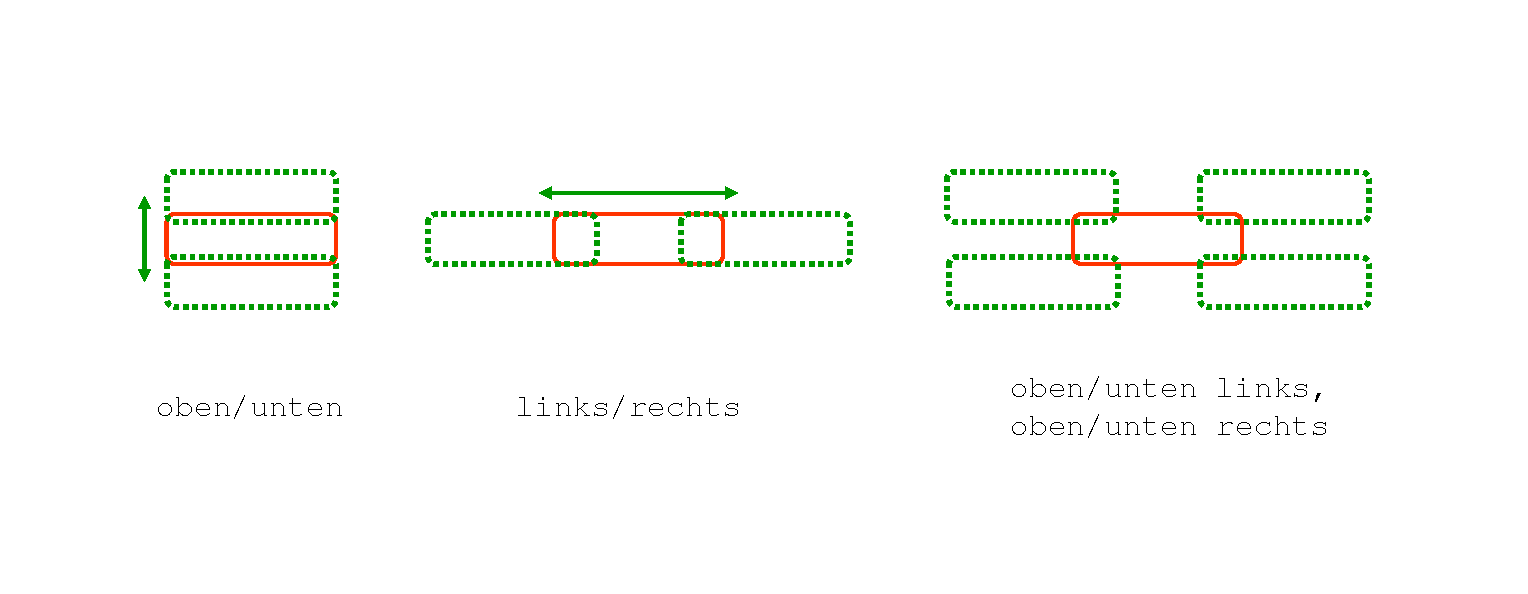
\includegraphics[width=0.75\textwidth]{img/bbox_shift}
\end{center}
\begin{table}[H]
\begin{tabular}{ccc}
\centering
\caption{Levenshtein-Distanz}
ohne Verschiebung        & mit Verschiebung         & mit Verschiebung
          \\
                         &                          & \&
Thresholding-Variierung \\
4.05 & 3.55 & 3.2
\end{tabular}
\end{table}
\end{frame}



\section{Learnings}

\begin{frame}{Learnings}
    \textbf{Erfolgreiches Programmieren im Projekt erfordert Rahmenbedingungen}
    \begin{itemize}
        \item[$\rightarrow$] Requirements festlegen (welche Pakete werden ben\"otigt, was muss installiert sein) $\rightarrow$ \texttt{requirements.txt}
        \item[$\rightarrow$] Versionskontrolle (in unserem Fall Git)\footnote{Besucht uns auf \url{https://github.com/cxan96/license_plate_detection}}
    \end{itemize}

    \textbf{Verbesserungen:}
    \begin{itemize}
        \item Die OCR-Pipeline ist manchmal noch recht fehleranf\"allig
              \begin{itemize}
                  \item[$\Rightarrow$] Schwellenwertverfahren verbessern
                  \item[$\Rightarrow$] Vielleicht Image Segmentation auch f\"ur OCR?
              \end{itemize}
        \item Geschwindigkeit kann noch verbessert werden
    \end{itemize}
\end{frame}



\begin{frame}[standout]
    Evaluator Results
\end{frame}

\begin{frame}{Evaluator Results}
    \begin{figure}
        \centering
        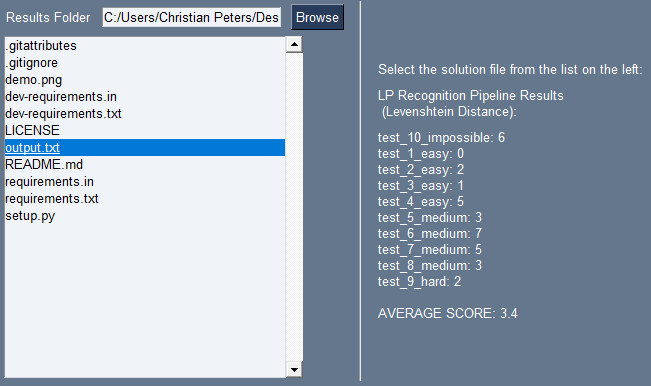
\includegraphics[width=\textwidth]{img/evaluator_results}
    \end{figure}
\end{frame}


\appendix

\begin{frame}[allowframebreaks]{Literatur}
  \nocite{*}
  \bibliography{literature}
  \bibliographystyle{abbrv}

\end{frame}

\end{document}
